\begin{enigme}[Nombres triangulaires]

Ci-dessous, les cinq premiers nombres « triangulaires » :

\begin{center} 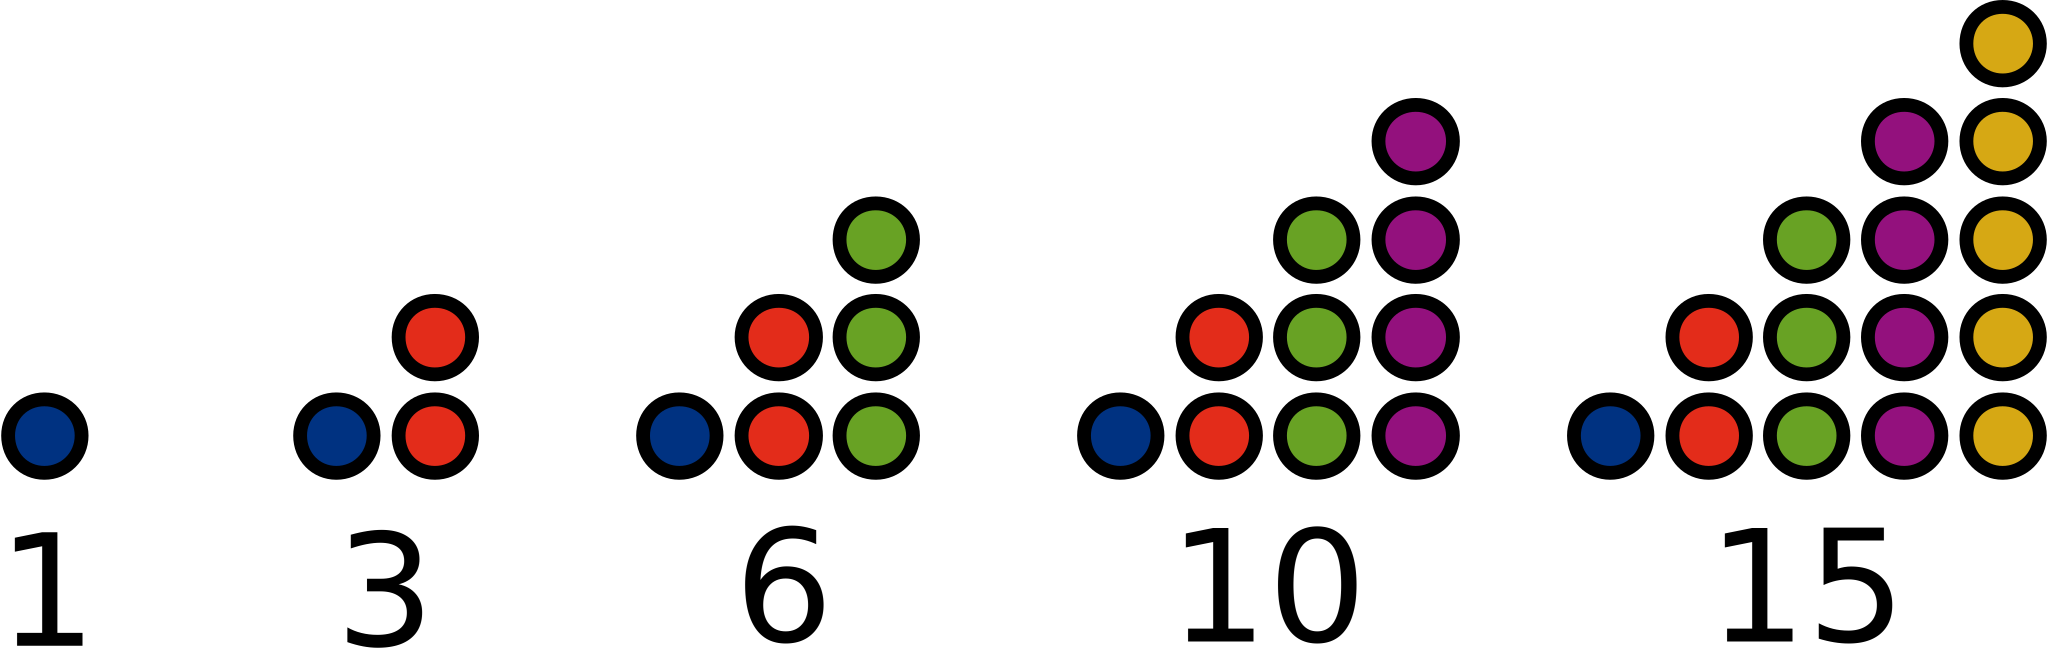
\includegraphics[width=5cm]{billes} \end{center} 

\begin{enumerate}
 \item Quel est le millième ?
 \item Que remarques-tu lorsque tu additionnes deux nombres triangulaires consécutifs ? 
 \end{enumerate}
 
 \end{enigme}
 
 \vspace*{2em}

\begin{enigme}[Geôle]
Dans un donjon, vingt cellules numérotées de 1 à 20 sont fermées à clé. Ces cellules s'ouvrent et se ferment en un tour de clé.

Alors que les prisonniers dorment à poings fermés, un premier gardien, les pensant ouvertes, met un tour de clé à toutes les cellules.

Peu après, un deuxième gardien met un tour de clé à toutes les cellules dont le numéro est multiple de 2.

Arrive ensuite un troisième gardien qui met un tour de clef à toutes les cellules dont le numéro est un multiple de 3 !

Et ainsi de suite...

Au final, vingt gardiens se sont succédés !

\begin{enumerate}
 \item Quels sont les numéros des cellules dont les prisonniers vont facilement pouvoir s'évader ?
 \end{enumerate}
 
\emph{Reprends le même problème avec 500 cellules et 500 passages de gardiens !! Justifie ta réponse.}
\end{enigme} 
